\documentclass[aspectratio=169,10pt]{beamer}

% Theme and appearance
\usetheme{Madrid}
\usecolortheme{default}
\setbeamertemplate{navigation symbols}{}
\setbeamertemplate{footline}[frame number]

% Packages
\usepackage[utf8]{inputenc}
\usepackage[T1]{fontenc}
\usepackage[english]{babel}
\usepackage{amsmath}
\usepackage{graphicx}
\usepackage{tikz}
\usepackage{xcolor}
\usepackage{listings}
\usepackage{fontawesome5}
\usepackage{tabularx}

% TikZ libraries
\usetikzlibrary{shapes,arrows,positioning,fit,calc,shadows,decorations.pathreplacing}

% Colors
\definecolor{attackred}{RGB}{220,50,50}
\definecolor{defensegreen}{RGB}{50,150,50}
\definecolor{warningorange}{RGB}{255,140,0}

% Custom commands
\newcommand{\mitm}{\textit{Man-in-the-Middle}}

% Title information
\title{Man-in-the-Middle (MITM) Attacks}
\subtitle{Principles, Examples and Defenses}
\author{Ahmed Dinari}
\institute{Project: Network Protocols - Attacks and Defenses}
\date{\today}

\begin{document}

% ============================================================
% SLIDE 1: Title
% ============================================================
\begin{frame}
  \titlepage
\end{frame}

% ============================================================
% SLIDE 2: Motivation / Scenario
% ============================================================
\begin{frame}{Motivation: What is MITM?}
  
  \begin{columns}[T]
    \begin{column}{0.48\textwidth}
      \small
      \textbf{Normal Communication:}
      \begin{itemize}\footnotesize
        \item Client $\leftrightarrow$ Server
        \item Direct connection
        \item Assumed confidentiality
      \end{itemize}
      
      \vspace{0.3em}
      \textbf{Attacker's Goal:}
      \begin{itemize}\footnotesize
        \item Position \textcolor{attackred}{between} the two
        \item Without being detected
        \item Intercept and manipulate
      \end{itemize}
      
      \vspace{0.3em}
      \textbf{Enables:}
      \begin{itemize}\footnotesize
        \item \faEye\ Eavesdropping
        \item \faEdit\ Data modification
        \item \faKey\ Credential theft
        \item \faArrowsAltH\ Redirection
      \end{itemize}
    \end{column}
    
    \begin{column}{0.48\textwidth}
      \begin{center}
        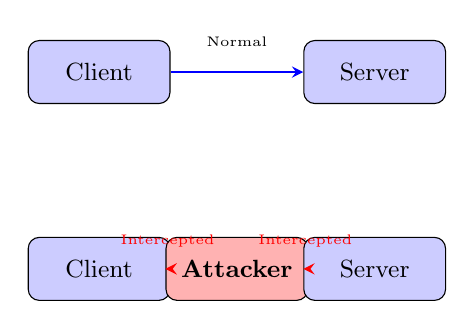
\begin{tikzpicture}[
          node distance=2cm,
          every node/.style={font=\small},
          box/.style={rectangle, draw, fill=blue!20, minimum width=1.8cm, minimum height=0.8cm, rounded corners},
          attacker/.style={rectangle, draw, fill=red!30, minimum width=1.8cm, minimum height=0.8cm, rounded corners},
          arrow/.style={->, >=stealth, thick}
        ]
          
          % Normal communication
          \node[box] (client1) at (0,2.5) {Client};
          \node[box] (server1) at (3.5,2.5) {Server};
          \draw[arrow, blue] (client1) -- (server1);
          \node[above, font=\tiny] at (1.75,2.7) {Normal};
          
          % MITM attack
          \node[box] (client2) at (0,0) {Client};
          \node[attacker] (attacker) at (1.75,0) {\textbf{Attacker}};
          \node[box] (server2) at (3.5,0) {Server};
          
          \draw[arrow, red, thick] (client2) -- (attacker);
          \draw[arrow, red, thick] (attacker) -- (server2);
          
          \node[above, font=\tiny, text=red] at (0.87,0.15) {Intercepted};
          \node[above, font=\tiny, text=red] at (2.62,0.15) {Intercepted};
          
        \end{tikzpicture}
      \end{center}
      
      \vspace{0.5em}
      \begin{alertblock}{Principle}
        If Alice thinks she's talking to Bob, but everything goes through Mallory $\rightarrow$ \textbf{Man-in-the-Middle}
      \end{alertblock}
    \end{column}
  \end{columns}
  
\end{frame}

% ============================================================
% SLIDE 3: Definition & Types of MITM
% ============================================================
\begin{frame}{What is a Man-in-the-Middle Attack?}
  
  \begin{block}{Definition}\small
    An \textbf{active} attack on the \textcolor{attackred}{confidentiality} and \textcolor{attackred}{integrity} of communications
  \end{block}
  
  \vspace{0.2em}
  
  \textbf{The Attacker:}
  \begin{itemize}\footnotesize
    \item Intercepts traffic
    \item Reads data
    \item Sometimes modifies content
  \end{itemize}
  
  \vspace{0.2em}
  
  \begin{columns}[T]
    \begin{column}{0.48\textwidth}
      \textbf{Common Types:}
      \begin{itemize}
        \item \textcolor{blue}{Passive MITM}
          \begin{itemize}
            \item Listening / sniffing
            \item No modification
          \end{itemize}
        \item \textcolor{attackred}{Active MITM}
          \begin{itemize}
            \item Modification
            \item Redirection
            \item Content injection
          \end{itemize}
      \end{itemize}
    \end{column}
    
    \begin{column}{0.48\textwidth}
      \textbf{Combines with:}
      \begin{itemize}
        \item ARP spoofing
        \item DNS spoofing
        \item Rogue Wi-Fi
        \item SSL stripping
        \item Certificate spoofing
      \end{itemize}
    \end{column}
  \end{columns}
  
\end{frame}

% ============================================================
% SLIDE 4: MITM in Network Model
% ============================================================
\begin{frame}{MITM in the Network Model}
  
  \begin{columns}[T]
    \begin{column}{0.55\textwidth}
      \footnotesize
      \textbf{Can target multiple layers:}
      
      \begin{itemize}\footnotesize
        \item \textbf{Link Layer (Layer 2)}
          \begin{itemize}\tiny
            \item ARP spoofing on LAN
            \item Malicious switch
          \end{itemize}
        
        \item \textbf{Network/Transport (L3-4)}
          \begin{itemize}\tiny
            \item Route hijacking (BGP)
            \item TCP hijacking
          \end{itemize}
        
        \item \textbf{Application (Layer 7)}
          \begin{itemize}\scriptsize
            \item Unencrypted HTTP
            \item Fake Wi-Fi portals
            \item Fraudulent TLS certificates
          \end{itemize}
      \end{itemize}
      
      \vspace{0.2em}
      
      \begin{alertblock}{In Practice}\footnotesize
        Modern MITM targets:
        \begin{itemize}\scriptsize
          \item Unsecured local networks
          \item Public Wi-Fi
          \item Unencrypted protocols
        \end{itemize}
      \end{alertblock}
    \end{column}
    
    \begin{column}{0.42\textwidth}
      \begin{center}
        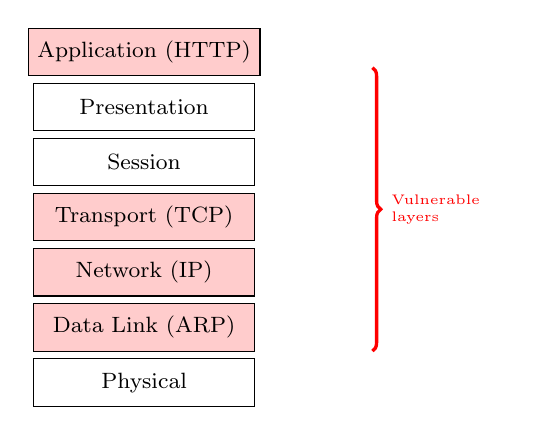
\begin{tikzpicture}[
          layer/.style={rectangle, draw, minimum width=2.8cm, minimum height=0.6cm, font=\footnotesize},
          vulnerable/.style={fill=red!20},
          secure/.style={fill=green!20}
        ]
          
          \node[layer, vulnerable] (app) at (0,0) {Application (HTTP)};
          \node[layer] (pres) at (0,-0.7) {Presentation};
          \node[layer] (sess) at (0,-1.4) {Session};
          \node[layer, vulnerable] (trans) at (0,-2.1) {Transport (TCP)};
          \node[layer, vulnerable] (net) at (0,-2.8) {Network (IP)};
          \node[layer, vulnerable] (link) at (0,-3.5) {Data Link (ARP)};
          \node[layer] (phys) at (0,-4.2) {Physical};
          
          % Bracket showing vulnerable layers
          \draw[red, very thick, decorate, decoration={brace, amplitude=3pt}] 
            (2.9,-0.2) -- (2.9,-3.8) node[midway, right=3pt, text width=1.5cm, font=\tiny] {Vulnerable layers};
            
        \end{tikzpicture}
      \end{center}
    \end{column}
  \end{columns}
  
\end{frame}

% ============================================================
% SLIDE 5: Example 1 - ARP Spoofing (How it works) + Technical Details
% ============================================================
\begin{frame}{Example 1: MITM on Local Network (ARP)}
  
  \begin{columns}[T]
    \begin{column}{0.48\textwidth}
      \textbf{How ARP Works:}
      \begin{itemize}\footnotesize
        \item ARP = Address Resolution Protocol
        \item Maps IP $\leftrightarrow$ MAC address
        \item Used on local networks (LAN)
        \item \textcolor{attackred}{\faExclamationTriangle\ No authentication!}
      \end{itemize}
      
      \vspace{0.2em}
      
      \textbf{The Attack:}
      \begin{enumerate}\footnotesize
        \item Attacker sends \textbf{fake ARP replies}
        \item Claims to be the router: \\
          \textit{``Router's IP has MY MAC''}
        \item Claims to be the victim: \\
          \textit{``Victim's IP has MY MAC''}
        \item \textbf{Result:} all traffic passes through attacker
      \end{enumerate}
      
      \vspace{0.15em}
      
      \begin{exampleblock}{Technical Detail}\scriptsize
        ARP is stateless - accepts unsolicited replies (gratuitous ARP). Cache poisoning persists until timeout (typically 2-20 min).
      \end{exampleblock}
    \end{column}
    
    \begin{column}{0.48\textwidth}
      \begin{center}
        \textbf{ARP Spoofing Scenario}
        
        \vspace{0.3em}
        
        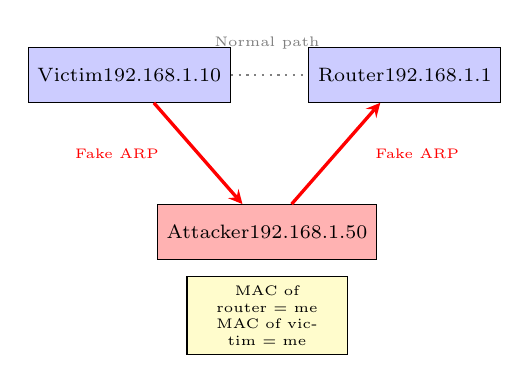
\begin{tikzpicture}[
          node distance=1.3cm,
          device/.style={rectangle, draw, fill=blue!20, minimum width=2cm, minimum height=0.7cm, font=\scriptsize},
          attacker/.style={rectangle, draw, fill=red!30, minimum width=2cm, minimum height=0.7cm, font=\scriptsize},
          arrow/.style={->, >=stealth, thick}
        ]
          
          \node[device] (victim) at (0,2) {Victim \\ 192.168.1.10};
          \node[device] (router) at (3.5,2) {Router \\ 192.168.1.1};
          \node[attacker] (attacker) at (1.75,0) {Attacker \\ 192.168.1.50};
          
          % Normal path (grayed out)
          \draw[dotted, gray, thick] (victim) -- (router);
          \node[above, font=\tiny, gray] at (1.75,2.2) {Normal path};
          
          % MITM path
          \draw[arrow, red, very thick] (victim) -- (attacker);
          \draw[arrow, red, very thick] (attacker) -- (router);
          
          \node[left, font=\tiny, text=red] at (0.5,1) {Fake ARP};
          \node[right, font=\tiny, text=red] at (3,1) {Fake ARP};
          
          % ARP messages
          \node[draw, fill=yellow!20, font=\tiny, text width=1.8cm, below=0.2cm of attacker, align=center] 
            {MAC of router = me\\MAC of victim = me};
          
        \end{tikzpicture}
      \end{center}
      
      \vspace{0.3em}
      
      \begin{block}{Note}\footnotesize
        No complex tools needed - protocol vulnerable by design
      \end{block}
    \end{column}
  \end{columns}
  
\end{frame}

% ============================================================
% SLIDE 6: ARP Attack Flow Diagram
% ============================================================
\begin{frame}{ARP Attack: Detailed Flow}
  
  \begin{center}
    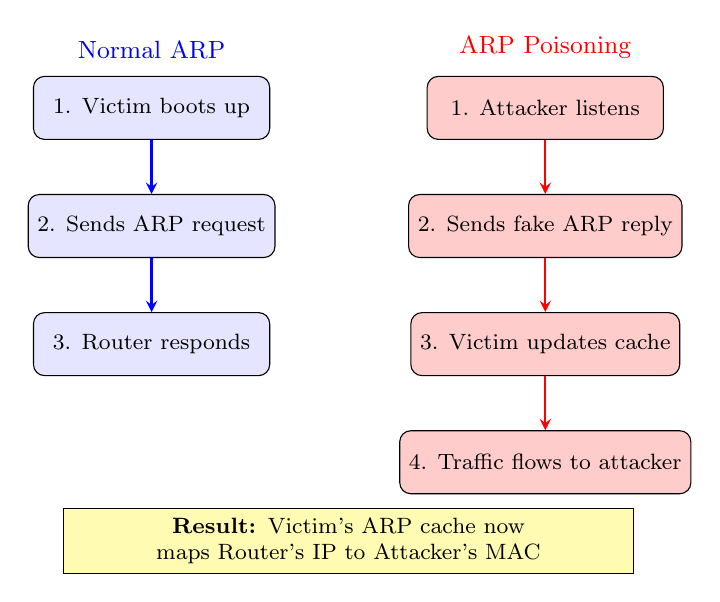
\begin{tikzpicture}[
      node distance=1.5cm,
      flowstep/.style={rectangle, draw, fill=blue!10, minimum width=3cm, minimum height=0.8cm, font=\footnotesize, rounded corners},
      attack/.style={rectangle, draw, fill=red!20, minimum width=3cm, minimum height=0.8cm, font=\footnotesize, rounded corners},
      arrow/.style={->, >=stealth, thick}
    ]
      
      % Normal flow
      \node[flowstep] (step1) at (0,3) {1. Victim boots up};
      \node[flowstep] (step2) at (0,1.5) {2. Sends ARP request};
      \node[flowstep] (step3) at (0,0) {3. Router responds};
      
      % Attack flow
      \node[attack] (attack1) at (5,3) {1. Attacker listens};
      \node[attack] (attack2) at (5,1.5) {2. Sends fake ARP reply};
      \node[attack] (attack3) at (5,0) {3. Victim updates cache};
      \node[attack] (attack4) at (5,-1.5) {4. Traffic flows to attacker};
      
      % Arrows normal
      \draw[arrow, blue] (step1) -- (step2);
      \draw[arrow, blue] (step2) -- (step3);
      
      % Arrows attack
      \draw[arrow, red] (attack1) -- (attack2);
      \draw[arrow, red] (attack2) -- (attack3);
      \draw[arrow, red] (attack3) -- (attack4);
      
      % Labels
      \node[above, font=\small, blue] at (0,3.5) {Normal ARP};
      \node[above, font=\small, red] at (5,3.5) {ARP Poisoning};
      
      % Result
      \node[draw, fill=yellow!30, font=\footnotesize, text width=7cm, align=center] at (2.5,-2.5) 
        {\textbf{Result:} Victim's ARP cache now maps Router's IP to Attacker's MAC};
      
    \end{tikzpicture}
  \end{center}
  
\end{frame}

% ============================================================
% SLIDE 7: ARP Defense
% ============================================================
\begin{frame}{Defense Against ARP-based MITM}
  
  \begin{columns}[T]
    \begin{column}{0.48\textwidth}
      \textbf{\textcolor{attackred}{Possible Consequences:}}
      \begin{itemize}\footnotesize
        \item \faEye\ Traffic reading
          \begin{itemize}\scriptsize
            \item Passwords in cleartext
            \item HTTP cookies
            \item Sensitive data
          \end{itemize}
        \item \faEdit\ Packet modification
          \begin{itemize}\scriptsize
            \item Redirect to fake sites
            \item Inject malicious code
            \item Alter data
          \end{itemize}
        \item \faUserSecret\ Session hijacking
      \end{itemize}
    \end{column}
    
    \begin{column}{0.48\textwidth}
      \textbf{\textcolor{defensegreen}{Concrete Defenses:}}
      
      \textbf{1. End-to-end encryption}
      \begin{itemize}\footnotesize
        \item \faLock\ HTTPS, SSH, VPN
        \item Makes traffic unreadable
      \end{itemize}
      
      \textbf{2. Network protections}
      \begin{itemize}\footnotesize
        \item Static ARP entries (critical)
        \item \textbf{Dynamic ARP Inspection} (DAI)
        \item Port Security on switches
        \item Network segmentation / VLANs
      \end{itemize}
      
      \textbf{3. Monitoring}
      \begin{itemize}\footnotesize
        \item ARP anomaly detection
        \item IDS/IPS (Intrusion Detection)
        \item Logs and alerts
      \end{itemize}
    \end{column}
  \end{columns}
  
  \vspace{0.5em}
  
  \begin{exampleblock}{Best Practice}\small
    \faCheckCircle\ Use encrypted protocols + network hardening
  \end{exampleblock}
  
\end{frame}

% ============================================================
% SLIDE 8: Example 2 - HTTP vs HTTPS (SSL Stripping)
% ============================================================
\begin{frame}{MITM on HTTP / HTTPS (SSL Stripping)}
  
  \begin{columns}[T]
    \begin{column}{0.48\textwidth}
      \textbf{Normal Operation:}
      \begin{itemize}\footnotesize
        \item \textbf{HTTP} = cleartext traffic
          \begin{itemize}\scriptsize
            \item No encryption
            \item No authentication
          \end{itemize}
        \item \textbf{HTTPS} = HTTP + TLS
          \begin{itemize}\scriptsize
            \item Encryption
            \item Server authentication
            \item Data integrity
          \end{itemize}
      \end{itemize}
      
      \vspace{0.2em}
      
      \textbf{Attack: SSL Stripping}
      \begin{enumerate}\scriptsize
        \item Victim visits \texttt{http://site.com}
        \item MITM intercepts
        \item MITM $\leftrightarrow$ Server: \textcolor{defensegreen}{HTTPS} \faLock
        \item MITM $\leftrightarrow$ Victim: \textcolor{attackred}{HTTP} \faUnlock
        \item Attacker reads/modifies everything!
      \end{enumerate}
      
      \begin{exampleblock}{Key Insight}\tiny
        Exploits initial HTTP connection before HTTPS redirect
      \end{exampleblock}
    \end{column}
    
    \begin{column}{0.48\textwidth}
      \begin{center}
        \textbf{SSL Stripping Scenario}
        
        \vspace{0.15em}
        
        \begin{tikzpicture}[
          node distance=1.8cm,
          device/.style={rectangle, draw, fill=blue!20, minimum width=1.8cm, minimum height=0.8cm, font=\scriptsize},
          attacker/.style={rectangle, draw, fill=red!30, minimum width=1.8cm, minimum height=0.8cm, font=\scriptsize},
          arrow/.style={->, >=stealth, very thick}
        ]
          
          \node[device] (victim) at (0,0) {Victim};
          \node[attacker] (mitm) at (2.5,0) {MITM};
          \node[device] (server) at (5,0) {Server \\ \texttt{https://}};
          
          % HTTP connection
          \draw[arrow, red] (victim) -- node[above, font=\tiny] {HTTP \faUnlock} (mitm);
          
          % HTTPS connection
          \draw[arrow, green!50!black] (mitm) -- node[above, font=\tiny] {HTTPS \faLock} (server);
          
          % Data flow
          \node[below=0.3cm of victim, font=\tiny, text width=1.5cm, align=center] 
            {Sends in cleartext};
          \node[below=0.3cm of mitm, font=\tiny, text width=1.5cm, align=center, text=red] 
            {Reads \& modifies};
          \node[below=0.3cm of server, font=\tiny, text width=1.5cm, align=center] 
            {Thinks secure};
          
        \end{tikzpicture}
      \end{center}
      
      \vspace{0.2em}
      
      \begin{alertblock}{Problem}\scriptsize
        Victim sees normal HTTP connection, no attack indication
      \end{alertblock}
      
      \begin{exampleblock}{Visual Clue}\scriptsize
        Missing padlock \faLock\ in address bar
      \end{exampleblock}
    \end{column}
  \end{columns}
  
\end{frame}

% ============================================================
% SLIDE 9: SSL/TLS Handshake vs MITM
% ============================================================
\begin{frame}{How SSL/TLS Protects Against MITM}
  
  \begin{columns}[T]
    \begin{column}{0.48\textwidth}
      \textbf{TLS Handshake (Simplified):}
      
      \vspace{0.15em}
      
      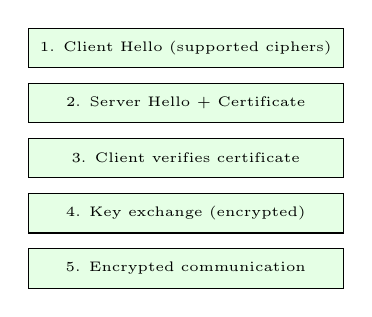
\begin{tikzpicture}[
        node distance=0.6cm,
        msg/.style={rectangle, draw, fill=green!10, minimum width=4cm, minimum height=0.5cm, font=\tiny}
      ]
        
        \node[msg] (msg1) at (0,0) {1. Client Hello (supported ciphers)};
        \node[msg] (msg2) at (0,-0.7) {2. Server Hello + Certificate};
        \node[msg] (msg3) at (0,-1.4) {3. Client verifies certificate};
        \node[msg] (msg4) at (0,-2.1) {4. Key exchange (encrypted)};
        \node[msg] (msg5) at (0,-2.8) {5. Encrypted communication};
        
      \end{tikzpicture}
      
      \vspace{0.3em}
      
      \begin{alertblock}{MITM Attempt}\footnotesize
        If attacker presents fake certificate, browser shows warning!
      \end{alertblock}
    \end{column}
    
    \begin{column}{0.48\textwidth}
      \textbf{Certificate Validation:}
      
      \begin{itemize}\footnotesize
        \item \textbf{Domain name} match
        \item \textbf{Certificate Authority} (CA) trust
        \item \textbf{Expiration} date
        \item \textbf{Signature} verification
        \item \textbf{Certificate chain} integrity
      \end{itemize}
      
      \vspace{0.15em}
      
      \textbf{Why it stops MITM:}
      
      \begin{itemize}\footnotesize
        \item Attacker can't forge valid certificate
        \item CA won't sign attacker's certificate for victim's domain
        \item Private key stays on legitimate server
        \item Browser validates entire chain
      \end{itemize}
      
      \vspace{0.3em}
      
      \begin{exampleblock}{Technical Note}\footnotesize
        TLS 1.3 provides forward secrecy (PFS) - even if server key compromised later, past sessions remain secure
      \end{exampleblock}
    \end{column}
  \end{columns}
  
\end{frame}

% ============================================================
% SLIDE 10: HTTP/HTTPS Defense
% ============================================================
\begin{frame}{Defense Against MITM on HTTP/HTTPS}
  
  \begin{columns}[T]
    \begin{column}{0.48\textwidth}
      \textbf{\textcolor{defensegreen}{1. Force HTTPS}}
      \begin{itemize}\footnotesize
        \item HTTP $\rightarrow$ HTTPS redirects server-side
        \item \textbf{HSTS} (HTTP Strict Transport Security)
          \begin{itemize}\scriptsize
            \item Forces browser to use HTTPS
            \item Prevents downgrade to HTTP
          \end{itemize}
        \item HSTS preload lists in browsers
      \end{itemize}
      
      \vspace{0.2em}
      
      \textbf{\textcolor{defensegreen}{2. Verify TLS Certificates}}
      \begin{itemize}\footnotesize
        \item Correct domain name
        \item Valid Certificate Authority
        \item Valid dates
        \item \textcolor{attackred}{\faExclamationTriangle\ NEVER ignore warnings!}
      \end{itemize}
    \end{column}
    
    \begin{column}{0.48\textwidth}
      \textbf{\textcolor{defensegreen}{3. Client Side}}
      \begin{itemize}\footnotesize
        \item Up-to-date browsers
        \item Check padlock \faLock\ before entering sensitive data
        \item Extensions: HTTPS Everywhere
        \item Avoid public Wi-Fi for sensitive data
      \end{itemize}
      
      \vspace{0.2em}
      
      \textbf{\textcolor{defensegreen}{4. For Applications}}
      \begin{itemize}\footnotesize
        \item \textbf{Certificate pinning}
          \begin{itemize}\footnotesize
            \item App only accepts specific certificates
            \item Prevents fraudulent certificates
          \end{itemize}
        \item Strict certificate validation
        \item No HTTP fallback
      \end{itemize}
    \end{column}
  \end{columns}
  
  \vspace{0.5em}
  
  \begin{exampleblock}{Golden Rule}\small
    \faCheckCircle\ \textbf{Always check HTTPS before entering:}
    Passwords, banking info, personal data
  \end{exampleblock}
  
\end{frame}

% ============================================================
% SLIDE 11: Example 3 - Wi-Fi Public (Rogue AP)
% ============================================================
\begin{frame}{MITM on Public Wi-Fi}
  
  \begin{columns}[T]
    \begin{column}{0.48\textwidth}
      \textbf{Typical Attack: Rogue Access Point}
      
      \vspace{0.2em}
      
      \textbf{Concept:}
      \begin{enumerate}\footnotesize
        \item Attacker creates fake Wi-Fi AP
        \item Same name (SSID) as legitimate network
          \begin{itemize}\footnotesize
            \item ``Starbucks WiFi''
            \item ``FreeWiFi''
            \item ``Hotel\_Guest''
          \end{itemize}
        \item Stronger signal than real AP
        \item Victims auto-connect
      \end{enumerate}
      
      \vspace{0.2em}
      
      \textbf{Attacker can:}
      \begin{itemize}\footnotesize
        \item \faEye\ Observe all traffic
        \item \faEdit\ Modify requests/responses
        \item \faUserSecret\ Create fake login portals (phishing)
        \item \faArrowDown\ Force downgrades (weak protocols)
      \end{itemize}
    \end{column}
    
    \begin{column}{0.48\textwidth}
      \begin{center}
        \begin{tikzpicture}[
          node distance=1cm,
          ap/.style={rectangle, draw, fill=blue!20, minimum width=1.8cm, minimum height=0.6cm, font=\tiny},
          rogue/.style={rectangle, draw, fill=red!30, minimum width=1.8cm, minimum height=0.6cm, font=\tiny},
          user/.style={circle, draw, fill=green!20, minimum size=0.6cm, font=\tiny}
        ]
          
          % Legitimate AP
          \node[ap] (legit) at (0,2.5) {Legitimate AP \\ \faWifi\ ``Cafe WiFi''};
          
          % Rogue AP
          \node[rogue] (rogue) at (0,0.8) {\textbf{Rogue AP} \\ \faWifi\ ``Cafe WiFi''};
          
          % Users
          \node[user] (user1) at (-2,1.8) {\faUser};
          \node[user] (user2) at (-2,0.3) {\faUser};
          \node[user] (user3) at (-2,1.2) {\faUser};
          
          % Connections to rogue
          \draw[->, red, thick] (user1) -- (rogue);
          \draw[->, red, thick] (user2) -- (rogue);
          \draw[->, red, thick] (user3) -- (rogue);
          
          % Internet
          \node[ap] (internet) at (2.5,1.5) {\faGlobe\ Internet};
          \draw[->, thick] (rogue) -- (internet);
          
          % Labels
          \node[font=\tiny, text=red] at (-2.5,2.2) {Victims};
          \node[font=\tiny, text width=1.5cm, align=center] at (1.2,0.2) {Traffic intercepted};
          
        \end{tikzpicture}
      \end{center}
      
      \vspace{0.3em}
      
      \begin{alertblock}{Danger}\footnotesize
        Users see no difference - same name, easy connection
      \end{alertblock}
      
      \vspace{0.3em}
      
      \begin{exampleblock}{Real Scenario}\footnotesize
        Café, airport, hotel - anywhere with public Wi-Fi
      \end{exampleblock}
    \end{column}
  \end{columns}
  
\end{frame}

% ============================================================
% SLIDE 12: Wi-Fi Security Comparison
% ============================================================
\begin{frame}{Wi-Fi Security: Evolution}
  
  \begin{center}
    \small
    \begin{tabular}{|l|c|c|c|l|}
      \hline
      \textbf{Protocol} & \textbf{Year} & \textbf{Encryption} & \textbf{Security} & \textbf{Status} \\
      \hline
      WEP & 1997 & RC4 (40-104 bit) & \textcolor{red}{Very Weak} & \textcolor{red}{Deprecated} \\
      \hline
      WPA & 2003 & TKIP & \textcolor{orange}{Weak} & \textcolor{orange}{Legacy} \\
      \hline
      WPA2 & 2004 & AES-CCMP & \textcolor{defensegreen}{Strong} & \textcolor{defensegreen}{Current} \\
      \hline
      WPA3 & 2018 & AES-GCMP & \textcolor{blue}{Very Strong} & \textcolor{blue}{Recommended} \\
      \hline
    \end{tabular}
  \end{center}
  
  \vspace{0.3em}
  
  \begin{columns}[T]
    \begin{column}{0.48\textwidth}
      \textbf{WPA2/WPA3 Features:}
      \begin{itemize}\footnotesize
        \item \textbf{WPA2-Personal (PSK)}
          \begin{itemize}\scriptsize
            \item Pre-shared key
            \item Good for home
          \end{itemize}
        \item \textbf{WPA2-Enterprise (802.1X)}
          \begin{itemize}\scriptsize
            \item RADIUS authentication
            \item Best for organizations
          \end{itemize}
      \end{itemize}
    \end{column}
    
    \begin{column}{0.48\textwidth}
      \textbf{WPA3 Improvements:}
      \begin{itemize}\footnotesize
        \item \textbf{SAE} authentication
          \begin{itemize}\scriptsize
            \item Resistant to offline attacks
          \end{itemize}
        \item \textbf{Forward secrecy}
        \item \textbf{192-bit security}
      \end{itemize}
    \end{column}
  \end{columns}
  
  \vspace{0.2em}
  
  \begin{alertblock}{Recommendation}\footnotesize
    Use WPA3 where available, minimum WPA2-Enterprise for businesses
  \end{alertblock}
  
\end{frame}

% ============================================================
% SLIDE 13: Synthesis & Best Practices
% ============================================================
\begin{frame}{Defense Summary \& Best Practices}
  
  \begin{columns}[T]
    \begin{column}{0.48\textwidth}
      \textbf{\textcolor{defensegreen}{Wi-Fi Defenses:}}
      
      \begin{itemize}\footnotesize
        \item \faLock\ \textbf{Use VPN}
          \begin{itemize}\scriptsize
            \item Encrypts all traffic
            \item Even on public Wi-Fi
          \end{itemize}
        
        \item \faWifi\ \textbf{Prefer secure Wi-Fi}
          \begin{itemize}\scriptsize
            \item WPA2/WPA3-Enterprise
            \item Avoid WEP, WPA
          \end{itemize}
        
        \item \faCog\ \textbf{Device configuration}
          \begin{itemize}\scriptsize
            \item Disable auto-connect
            \item Verify network name
          \end{itemize}
      \end{itemize}
    \end{column}
    
    \begin{column}{0.48\textwidth}
      \textbf{\textcolor{defensegreen}{Overall Protection:}}
      
      \begin{block}{MITM Exploits:}\scriptsize
        \begin{itemize}\tiny
          \item Lack of encryption
          \item Implicit trust
          \item User negligence
        \end{itemize}
      \end{block}
      
      \begin{exampleblock}{Key Measures}\scriptsize
        \begin{enumerate}\tiny
          \item \textbf{Encryption:} HTTPS, SSH, TLS, VPN
          \item \textbf{Authentication:} Valid certificates
          \item \textbf{Network hardening:} Secure switches, WPA3
          \item \textbf{Awareness:} User training
        \end{enumerate}
      \end{exampleblock}
    \end{column}
  \end{columns}
  
  \begin{alertblock}{Conclusion}\scriptsize
    Defense in depth: Encryption + Authentication + Hardening + Awareness
  \end{alertblock}
  
\end{frame}

% ============================================================
% SLIDE 14: Live Demo (Windows Lab)
% ============================================================
\begin{frame}{Live Demo (Windows Lab)}
  \footnotesize
  \textbf{Goal:} show MITM in a safe, isolated lab on Windows (no real network impact)

  \vspace{0.2em}

  \begin{columns}[T]
    \begin{column}{0.52\textwidth}
      \textbf{Lab Setup}
      \begin{itemize}\scriptsize
        \item Host: Windows + WSL2 (Ubuntu) + Wireshark/Npcap
        \item Two VMs on Host-Only / Private vSwitch
        \item IP plan example: \texttt{192.168.56.1} (gateway VM), \texttt{.101} (victim), \texttt{.200} (attacker)
        \item Do this only in the lab network
      \end{itemize}

      \vspace{0.2em}

      \textbf{Traffic Capture}
      \begin{itemize}\scriptsize
        \item Start Wireshark on host/attacker interface
        \item Filter: \texttt{http} (for cleartext) or \texttt{tcp.port==8080} (if using mitmproxy)
      \end{itemize}
    \end{column}

    \begin{column}{0.46\textwidth}
      \textbf{Attack Steps (WSL2)}
      \begin{enumerate}\scriptsize
        \item \texttt{sudo apt update \&\& sudo apt install dsniff mitmproxy}
        \item Enable forwarding: \texttt{sudo sysctl -w net.ipv4.ip\_forward=1}
        \item ARP poison both ends: \\
          \texttt{sudo arpspoof -i eth0 -t 192.168.56.101 192.168.56.1} \\[-0.3em]
          \texttt{sudo arpspoof -i eth0 -t 192.168.56.1   192.168.56.101}
        \item (HTTP sniff) Browse HTTP from victim; view in Wireshark
        \item (SSL strip) Redirect HTTP to mitmproxy: \\
          \texttt{sudo iptables -t nat -A PREROUTING -p tcp --dport 80 -j REDIRECT --to-port 8080} \\[-0.3em]
          \texttt{mitmproxy --mode transparent --showhost}
      \end{enumerate}

      \vspace{0.2em}
      \textbf{Safety}
      \begin{itemize}\scriptsize
        \item Keep lab isolated; disable when done: \texttt{sudo iptables -t nat -F}
        \item HTTPS sites will warn on bad certs; demo that warning = protection
      \end{itemize}
    \end{column}
  \end{columns}

\end{frame}

% ============================================================
% SLIDE 14: Real-World Case Study
% ============================================================
\begin{frame}{Real-World Example: Public Wi-Fi Attack (2015)}
  
  \textbf{Scenario: Airport Wi-Fi MITM}
  
  \vspace{0.2em}
  
  \begin{columns}[T]
    \begin{column}{0.48\textwidth}
      \textbf{What Happened:}
      \begin{enumerate}\footnotesize
        \item Attacker set up rogue AP at major airport
        \item SSID: ``Airport\_Free\_WiFi'' (looked legitimate)
        \item 200+ users connected in 3 hours
        \item SSL stripping used on banking sites
        \item Credentials harvested from HTTP sites
      \end{enumerate}
      
      \vspace{0.15em}
      
      \textbf{Attack Chain:}
      \begin{itemize}\footnotesize
        \item \textbf{Layer 2:} Rogue AP
        \item \textbf{Layer 3-4:} Traffic routing through attacker
        \item \textbf{Layer 7:} SSL stripping, DNS spoofing
      \end{itemize}
    \end{column}
    
    \begin{column}{0.48\textwidth}
      \textbf{Why It Succeeded:}
      \begin{itemize}\footnotesize
        \item Users trusted ``free'' Wi-Fi
        \item No VPN usage
        \item Many sites still used HTTP
        \item Users ignored certificate warnings
        \item Auto-connect enabled
      \end{itemize}
      
      \vspace{0.15em}
      
      \textbf{What Could Have Prevented It:}
      \begin{itemize}\footnotesize
        \item \faCheckCircle\ VPN mandatory for public Wi-Fi
        \item \faCheckCircle\ HSTS on all websites
        \item \faCheckCircle\ User awareness training
        \item \faCheckCircle\ Disable auto-connect
        \item \faCheckCircle\ Verify network legitimacy
      \end{itemize}
    \end{column}
  \end{columns}
  
  \vspace{0.2em}
  
  \begin{exampleblock}{Lesson Learned}\footnotesize
    \textbf{Defense in depth:} Multiple layers of protection needed. One missing layer = vulnerability.
  \end{exampleblock}
  
\end{frame}

% ============================================================
% FINAL SLIDE: Questions
% ============================================================
\begin{frame}[plain]
  \begin{center}
    \Huge \textbf{Thank You!}
    
    \vspace{1em}
    
    \Large Questions?
    
    \vspace{2em}
    
    \normalsize
    \faEnvelope\ ahmed.dinari@polytechnicien.tn
    
    \vspace{0.5em}
    
    \faGithub\ github.com/amedo007-poly
    
    \vspace{1.5em}
    
    \small
    \textit{``Security is not a product, but a process''} \\
    \textit{- Bruce Schneier}
  \end{center}
\end{frame}

\end{document}
